\documentclass{article}
\usepackage{graphicx}
\graphicspath{{./imgs}}
\begin{document}
\section*{Problem 2}
\subsection*{a.}
\begin{enumerate}
  \item The pipeline for this project is:
        1024x1024 Images $\rightarrow$ Resize to 64x64 $\rightarrow$ Augment the data by adding mirrored
        images to the dataset $\rightarrow$ Train VAE $\rightarrow$ Plot the images across the latent
        space.
  \item Vanilla AE
  \item 2D latent space was chosen since it is easy 
        to show the latent space and
        do latent space arithmetic or transformations.
  \item For the real life legos, converting and augmenting data takes 
        about 1 minute and training takes 14 seconds.
        For the rendered legos, 1.5 minutes and 1.7 minutes.
  \item I was unable to do 1024x1024 training since I didn't have enough vram for it,
        but for the repo that I cloned, the highest dimesion that was able to still
        be graphed was 64x64. So we had to lower the resolution and we decided on
        64x64 since it was still relatively fast to train and it was the biggest
        we can do.
  \item The biggest challenge was trying to get the dataset to actually
        work with the VAE that was found. What was really helpful was
        looking at the shapes of the numpy arrays if you get operation errors.
        In addition, I wasn't sure how to get the graphs working with colors
        so I decided to do only greyscale instead.
\end{enumerate}

\subsection*{b. Passing Original Images Through VAE (Real Legos)}
\begin{center}
  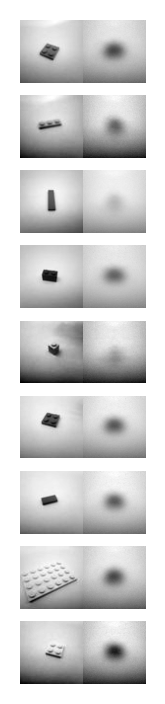
\includegraphics[scale=1]{10_original-lego-dataset}
\end{center}

The VAE managed to capture the color of the pieces,
however the shape of the pieces were lost.
There is one outlier which is the large float white piece;
that piece's color and shape were not captured.

\subsection*{c. Graphs of the Latent Space (Real Legos)}

Here is a plot of the dataset on the latent space:

\begin{center}
  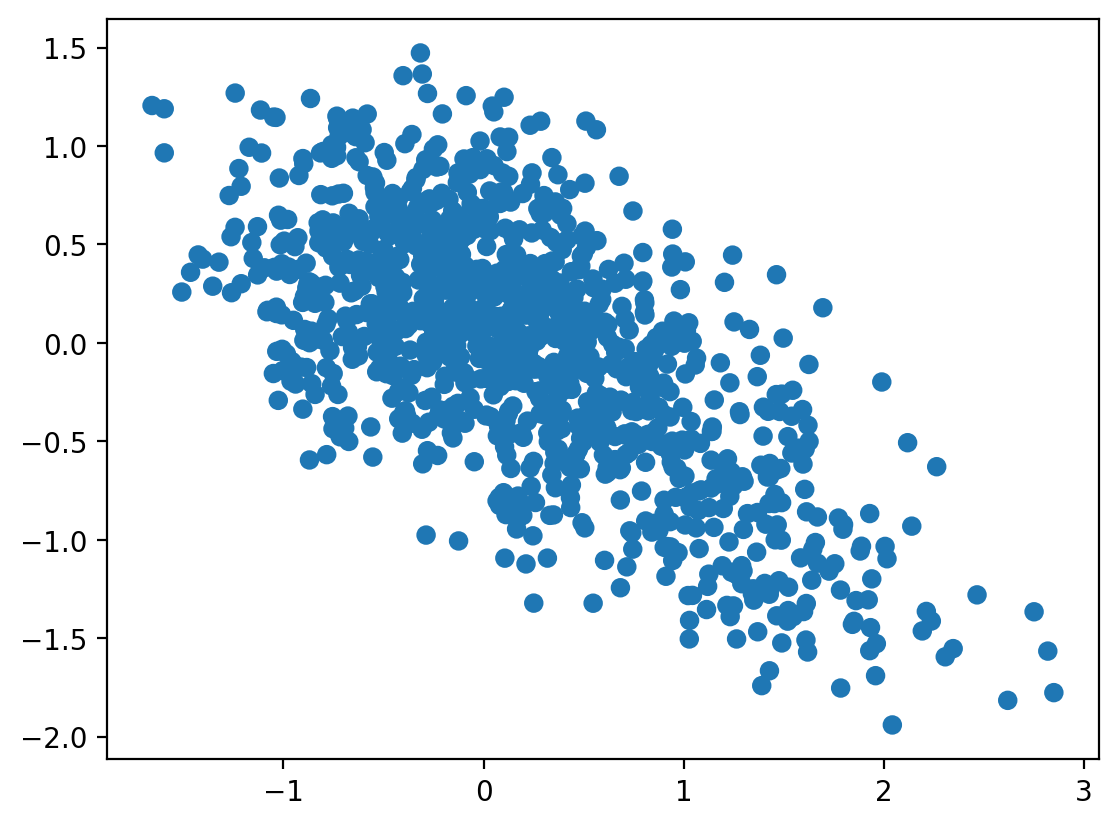
\includegraphics[scale=0.75]{latent_space-lego-dataset}
\end{center}

Here is a plot of images sampled across the latent space:

\begin{center}
  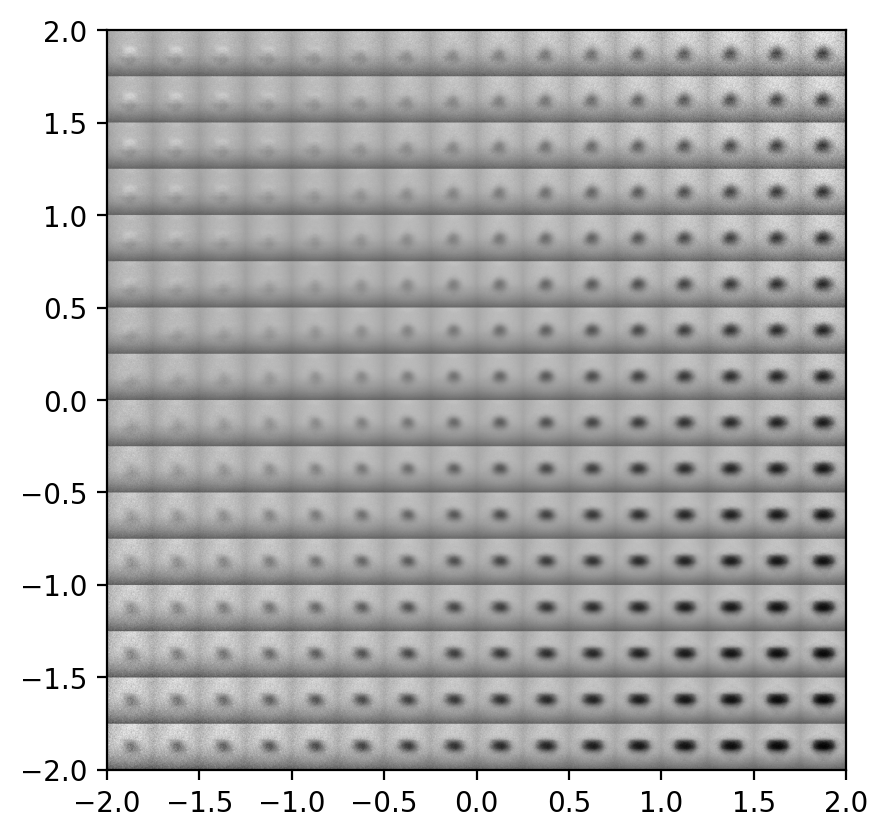
\includegraphics[scale=1]{latent_space_examples-lego-dataset}
\end{center}

The area nearby the origin in latent space is very blurry and hard
to distinguish between the lego and the background. The farther
out you go from the origin, the more the lego looks like but
there is more noise added to the image.

The two features that the VAE were able to pick up on were the color
of the lego and a very general shape or rotation of the piece.

I think the images are very reasonable given the data.

\subsection*{d. Interpolation of Two Places in Latent Space (Real Legos)}
\begin{center}
  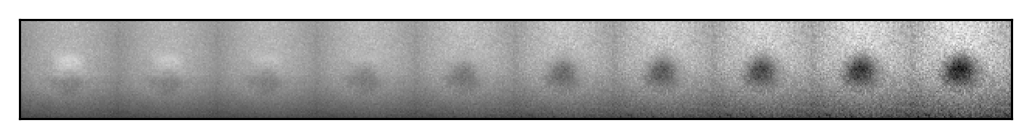
\includegraphics[scale=0.9]{interpolation-lego-dataset}
\end{center}

I took two points in the latent space (-2, 2) to (2, 2) and interpolated
the space between these points with the VAE.


\subsection*{b. Passing Original Images Through VAE (Rendered Legos)}
\begin{center}
  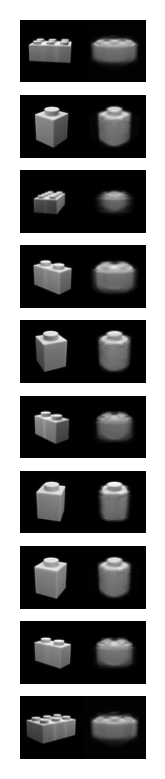
\includegraphics[scale=1]{10_original-lego-blender-4}
\end{center}

Compared to the real legos, the VAE managed to better capture
the overall shape of the legos. 
This is probably due to the more consistent framing of the legos
in the center of the image.
However, some of the legos when
look blurry as if it VAE were rotating the lego.

\subsection*{c. Graphs of the Latent Space (Rendered Legos)}

Here is a plot of the dataset on the latent space:

\begin{center}
  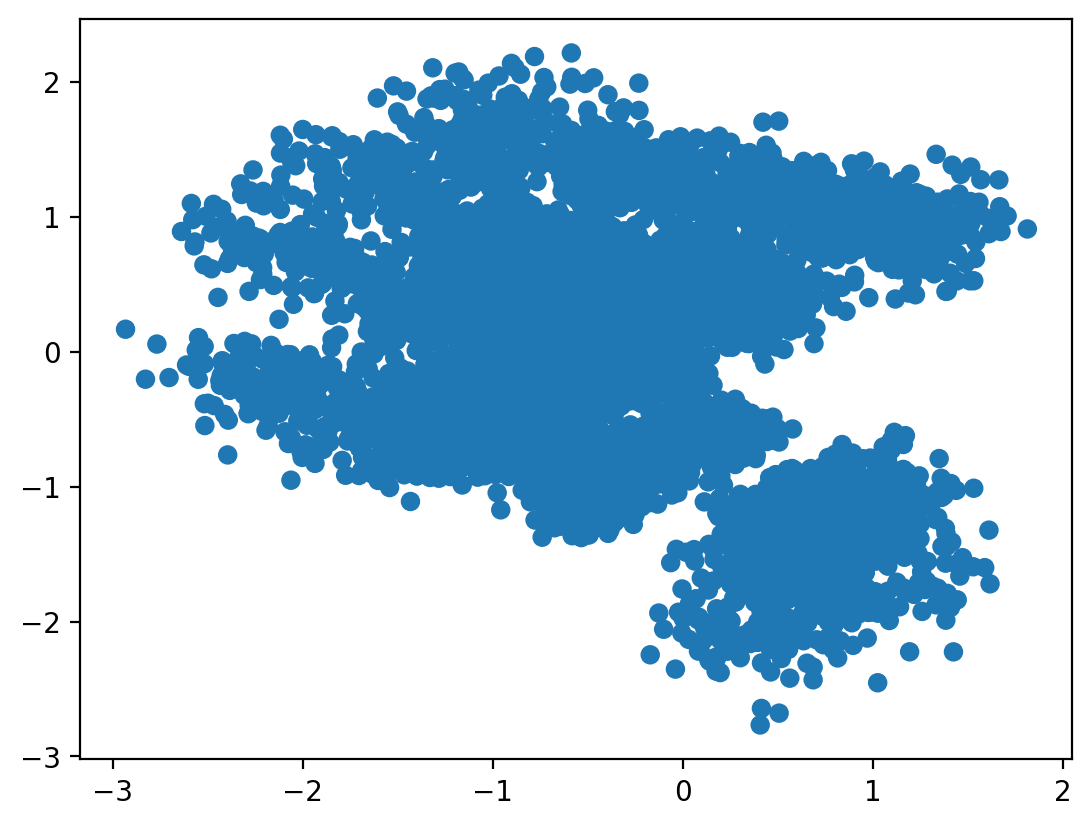
\includegraphics[scale=0.75]{latent_space-lego-blender-4}
\end{center}

Here is a plot of images sampled across the latent space:

\begin{center}
  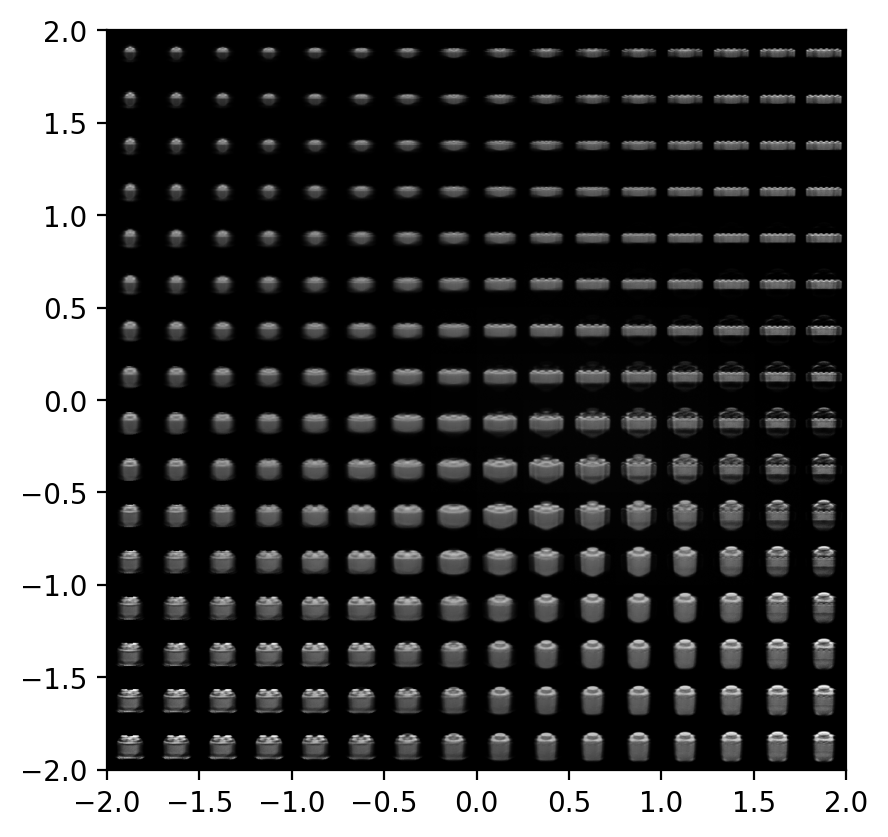
\includegraphics[scale=1]{latent_space_examples-lego-blender-4}
\end{center}

Compared to the latent space of the real legos, there are clear
areas where different types of bricks are located in the latent space.
Like the other VAEs that were demonstrated in the classroom,
thee are regions in the space where the VAE is blending between two or
more different types of bricks.

The features that the VAE were able to pick up on were
the type of bricks (1x1, 2x2, 2x4, 2x4). Since there
wasn't very much in difference in the colors of the bricks,
they are all the same greyish color.

I think the images are very reasonable given the data.

\subsection*{d. Interpolation of Two Places in Latent Space (Rendered Legos)}
\begin{center}
  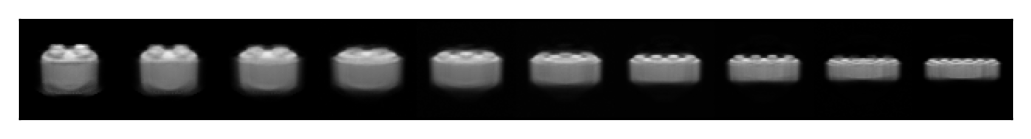
\includegraphics[scale=0.9]{interpolation-lego-blender-4}
\end{center}

I took two points in the latent space (-1, -1) to (1, 1) and interpolated
the space between these points with the VAE.

% We had an idea to render some lego bricks in blender and use those to train
% a VAE to try and get better results.

\end{document}